\chapter{Implementation}

\section{Meta Model and Instantiation}
Our system has a simple meta model for describing (nested) classes and their methods. The graphical user interface operates exclusively on the meta model and makes changes to it. The meta model can then be instantiated to generate the actual classes. When changes to the meta model are made, these changes can also be applied to already existing instantiations of the model, allowing giving programmers the feeling of working with a live system.

\paragraph{Smalltalk-80 Class/Meta Model}
Squeak already comes with a meta model: objects are instances of a classes, consequently, classes are also instances of a class. In Smalltalk, every class is an instance of its own meta class, which is in turn instance of \texttt{Metaclass}.

Our system allows class generation at runtime: class generator methods generate classes along with their respective meta classes. Therefore, we need a specification/blueprint that describes how a class generator method should construct a class. At first glance, it might seem logical to use meta classes; after all, a meta class is the class of a regular (non-meta) class and classes are instance generators. However, meta classes cannot be used as class object generators in a way required by our system for two reasons.

Firstly, meta classes do not have any information about their non-meta class counterpart: for example, they do not know anything about their instance methods or their instance variables. Instantiating a meta class would not generate a functional class object, which is why Smalltalk prohibits generating new instances of a meta class. In fact, the class \texttt{ClassBuilder} is used to create new classes and it always creates class objects alongs with their meta class objects.

Secondly, our system supports defining methods on the instance side and on the class side. Consequently, we do not only need to generate class object but also meta class objects. All meta classes are an instance of \texttt{Metaclass}. But if we wanted to generate different meta classes, we would need a different \texttt{Metaclass} class, each of which generates its corresponding meta class. In some programming languages, the instance-of chain carries on infinitely; Ruby is an example. However, in Smalltalk, every meta class is an instance of \texttt{Metaclass} and this is where the instance-of chain recurses: \texttt{Metaclass} is an instance of \texttt{Metaclass class}, which is an instance of \texttt{Metaclass}.

For this reason, we cannot use the Smalltalk-80 meta model to generate new classes on the fly and use our own simple meta model instead.

\paragraph{Nested Classes Meta Model}
Figure~\ref{fig:impl_meta_model} shows the meta model in our system. The meta model is built around specifications: there are specifications for classes, meta classes, and methods. A specification describes how its corresponding object is built. \texttt{ClassSpecification}s generate classes, \texttt{MetaclassSpecification}s generate meta classes, and \texttt{MethodSpecification}s generate methods. Since classes cannot exist without their respective meta classes, a class specification is always linked with its meta class specification and vice-versa. When a class specification is instantiated, the system generates both the class and the meta class. Meta class specifications cannot be instantiated.

\begin{figure}
	\centering
	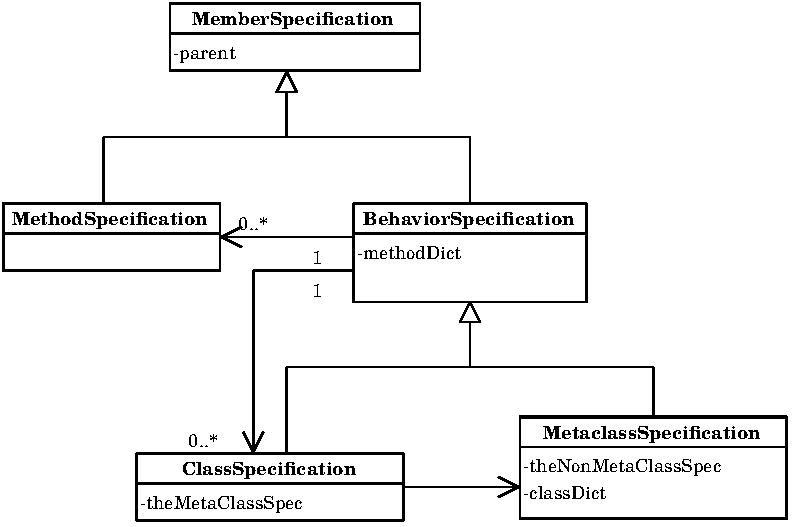
\includegraphics[scale=1]{metamodel.pdf}
	\caption{Meta Model for Nested Classes}
	\label{fig:impl_meta_model}
\end{figure}

\paragraph{Class Specifications}
A class specification describes classes. It has a collection of \texttt{MethodSpecification}s, representing instance methods of the class. Upon instantiation, all method specifications are instantiated within the target class. For every class specification, there is a corresponding method specification containing the source code of the class generator method in the parent's method dictionary. This method specification determines (when executed in the running system) to which class the methods will be added (\emph{target class}). Top-level classes are an exception: they are always a new subclass of the class \texttt{Module}.

\paragraph{Meta Class Specification}
A meta class specification describes meta classes. It has a collection of \texttt{MethodSpecification}s, representing class methods of the class (i.e., instance methods of the meta class). Upon instantiation, all method specifications are instantiated within the targer class' meta class. Consequently, meta classes do not method specifications associated with.

However, meta classes can have nested classes of their own. For every class defined in a meta class, there is a corresponding method specification present in the method dictionary (see previous paragraph).

\paragraph{Method Specification}
A method specification describes methods. It contains the source code of the method and stores information necessary for class caching and UI metadata. Whenever a method specification is instantiated, the method source code is compiled in the target class. 

Note, that different byte code must be generated for different target classes: for example, instance variable reads and write are compiled to parameterized\footnote{There are separate bytecodes for reading the first or second instance variable etc.} \texttt{pushRcvr:} and \texttt{popIntoRcvr:} bytecodes, where instance variables are referenced with their index\footnote{The first instance variable has index 0, second index variable has index 1, etc.}. In addition, the \texttt{outer} and the \texttt{enclosing} keyword must be bound to different method literals, depending on the lexical scope of the class.

\paragraph{Class Initialization}

accessor methods and generator methods, lazy initialization

\section{Anonymous Classes and Subclass Generation}

\section{\texttt{thisOuter} and \texttt{thisScope}}

\section{Class Updates}
using instances weak array on specification

\section{Integration in Squeak}

\subsection{Module Repository}
replacement for Smalltalk dict

\subsection{IDE Support}
works in workspace, test runner. How to write tests? New system browser

\subsection{Debugger}
shows slightly different code (thisContext automatically inserted, generator methods)